% Provenance (never printed): see sources/outline_sources.md (Year 1: the carbonate factory;
% reefs and platforms; pelagic oozes and the carbonate compensation depth; siliceous oozes;
% evaporite sequences). Exercise and problem values in the Book 3 scratch calculator
% calc/ch22.py; figure data from figdata/bachelor-1/evaporation.py and ccd_flank.py.
% Calcite, aragonite and dolomite are ch. 7's; the depth--age law ch. 13's; salinity Book 1's
% (g8); limestone Book 1's (g6, prose); the carbonate system and alkalinity the chemistry and
% biology books' (recalled, never defined). The subsidence of volcanic islands under reefs is
% the Year 2 volume's (oceanic islands); diagenesis (dolomitisation, chert, gypsum to
% anhydrite) is ch. 23's; upwelling ch. 29's.
\chapter{الرسوبيات الكربوناتية والسيليسية والتبخّرية}\label{ch:b1:chemical-biogenic-sediments}

صفائح الطباشير البيضاء المتقابلة عبر البحر الضيّق بين إنجلترا وفرنسا تبدو من أكثر الصخور عاديّةً. لكنها تحت المجهر الإلكتروني تتكوّن من عدد لا يُحصى من صفائح الكالسيت الصغيرة، خلّفتها طحالب وحيدة الخلية كانت تعوم في البحر الذي غطّى المنطقة. \omterm{def:b1:chemical-biogenic-sediments:reef}{والشعاب المرجانية} التي تُرى من قارب هي القصة نفسها على الطرف الآخر من السلّم: حجر كلسي قيد التكوّن، تبنيه المرجانيات والطحالب، فتأخذ الكالسيوم والكربونات من الماء وتحوّلهما حجرًا. وليست كل الرسوبيات منقولة؛ فكثير منها يتكوّن حيث يقع، بفعل كائنات حيّة أو بفعل الماء نفسه وهو يتبخّر. يتتبّع هذا الفصل العائلات الثلاث الكبرى لهذه الرسوبيات، وهي الكربونات، والرسوبات السيليسية الناعمة \omterm{def:b1:chemical-biogenic-sediments:evaporite}{والرسوبات التبخّرية}، من كيمياء البحر الذي يغذّيها إلى الصخور التي تتركها.

\begin{recall}
الحجر الكلسي صخر رسوبي مكوّن من الكالسيت، غالبًا من الأصداف، ويفوّر في الحمض المخفّف (الكتاب الأول، الصف السادس). والكالسيت والأراغونيت هما شكلان بلوريان ل\ce{CaCO3}، كثافتهما \qty{2.71}{g.cm^{-3}} و\qty{2.93}{g.cm^{-3}}، والدولوميت \ce{CaMg(CO3)2}، كثافته \qty{2.84}{g.cm^{-3}}، وهو كربونات الكالسيوم والمغنيسيوم (\cref{ch:b1:rock-forming-minerals}). وملوحة ماء البحر هي كتلة الملح المذاب في كيلوغرام منه (الكتاب الأول، الصف الثامن). وفي الماء، يرتبط ثاني أكسيد الكربون وأيون الهيدروجين الكربوني وأيون الكربونات بتوازنات حمض-قاعدة، والقلوية تقيس القواعد القادرة على امتصاص أيونات الهيدروجين (كتب الكيمياء)؛ ونظام الكربونات في المحيط يشارك في دورة الكربون (كتب الأحياء). وقاع البحر يعمق مع العمر وفق $d = d_r + C\sqrt t$ (\cref{thm:b1:rifts-ridges-margins:depth-age}).
\end{recall}
% ledger: webmineral:polymorphs, hom:calcite, webmineral:others

\section{مصنع الكربونات}\label{sec:b1:chemical-biogenic-sediments:factory}

تحتوي مياه البحر على الكالسيوم والكربون غير العضوي المذاب، معظمه في صورة بيكربونات الهيدروجين. ويتكوّن منهما كربونات الكالسيوم بالتفاعلين
\[
\ce{Ca^2+ + 2 HCO3- -> CaCO3 + CO2 + H2O}, \qquad
\ce{Ca^2+ + CO3^2- -> CaCO3},
\]
الأول يُطلق جزيءً من ثاني أكسيد الكربون مقابل كل وحدة كربونات تترسّب. والمياه السطحية الدافئة في المناطق الاستوائية فوق مشبعة بكربونات الكالسيوم، لكنها نادرًا ما تترسّب بذاتها: فمعظمها تصنعه الكائنات الحيّة، التي تدفع الطاقة لبناء أصدافها وهياكلها، وتتحكّم في \omterm{def:b1:rock-forming-minerals:mineral}{المعدن} الذي تستعمله. فالمرجانيات والطحالب الخضراء تبني الأراغونيت؛ والطحالب الحمراء والفورامينيفيرا الكثيرة تبني الكالسيت، بعضه غنيّ بالمغنيسيوم؛ والرخويات تستعمل أحدهما أو كليهما.

\begin{definition}[مصنع الكربونات]\label{def:b1:chemical-biogenic-sediments:factory}
\emph{مصنع الكربونات}\index{مصنع الكربونات} في بحر ما هو مجموعة الكائنات والعمليات التي تُنتج رسوب كربونات الكالسيوم حيث يوجد، بدل أن يُجلب من مكان آخر. ومنتجاته الحبيبات الهيكلية (أصداف وهياكل كاملة أو مكسورة)، والطين الكربوناتي، والحبيبات المغلّفة، والأُطر الصلبة \omterm{def:b1:chemical-biogenic-sediments:reef}{للشعاب المرجانية}.
\end{definition}

أغنى المصانع يعمل في المياه الدافئة الصافية الضحلة المشمسة، بعيدًا عن طين الأنهار الذي يدفن المنتجين ويعتّم الضوء الذي تحتاجه الطحالب. ويتكوّن رسوبه من قاع البحر نفسه: حطام المرجان والطحالب، وأصداف الرخويات والفورامينيفيرا وحيدة الخلية التي تعيش في القاع، وإبر الأراغونيت التي تطرحها الطحالب الخضراء، وهي تترسّب طينًا كلسيًّا. وحيث يكون الماء مضطربًا ومشبعًا، تكتسي الحبيبات التي تدحرجها الأمواج والمدّ طبقات من الكربونات، طبقةً فوق طبقة، حول نواة، هي حبيبة رمل أو شظية صدف، فتصير أويدات كروية (\cref{def:b1:chemical-biogenic-sediments:reef}). ويعمل مصنع ثانٍ في المحيط المفتوح، بعيدًا عن أي شاطئ: فالعوالق التي تعيش في الطبقة السطحية المشمسة تبني أصدافًا وصفائح كالسيتية دقيقة تتساقط إلى قاع البحر العميق (\cref{sec:b1:chemical-biogenic-sediments:oozes}).
% ledger: og:carbonates

وتُقاس سرعة بناء المصنع بميزانيته الكربوناتية، أي كتلة الكربونات المنتجة والمحفوظة في مكانها كل سنة على متر مربّع، بعد الخسائر بفعل الكائنات الحافرة والرعّاة والأمواج. وتتحوّل هذه الميزانية إلى معدّل نمو رأسي بتوازن كتلي.

\begin{proposition}[التراكم من ميزانية كربوناتية]\label{prop:b1:chemical-biogenic-sediments:accretion}
ليحتفظ قاع بحر في مكانه بالكتلة الصافية $G$ من كربونات الكالسيوم لكل وحدة مساحة ولكل وحدة زمن، كرسوب حبيباته الصلبة كثافتها $\rho_s$، ومساميّته، أي الكسر من حجمه الذي تشغله المسامات، هي $\phi$. فيرتفع القاع بالمعدّل
\[
a = \frac{G}{\rho_s\,(1-\phi)}.
\]
\end{proposition}

\begin{proof}
في الزمن $\mathrm dt$ تستقبل وحدة المساحة الكتلة $G\,\mathrm dt$ من الكربونات الصلبة، التي تملأ حجم $G\,\mathrm dt/\rho_s$ من الحبيبات. وهذه الحبيبات تشكّل الكسر $1-\phi$ من الطبقة الجديدة، فسمكها إذن $G\,\mathrm dt/(\rho_s(1-\phi))$. والقسمة على $\mathrm dt$ تعطي $a$.
\end{proof}

الكثافة الحجمية الجافّة للرسوب هي $\rho_s(1-\phi)$. وعلى شعاب أرخبيل تشاغوس في المحيط الهندي، قاست 28 شعابًا في 2015 ميزانيةً متوسطها \qty{3.7}{kg} من \ce{CaCO3} لكل متر مربّع في السنة، وكانت الشعاب التي تهيمن عليها مرجانيات \emph{Acropora} المتفرّعة \qty{8.4}{kg}، وتنمو بنحو \qty{4.2}{mm} في السنة؛ ومع المبرهنة يعني هذان العددان معًا كثافة حجمية جافّة \qty{2000}{kg.m^{-3}}، أي أن إطار الشعاب فيه نحو ثلث حجمه مسامات (\cref{exo:b1:chemical-biogenic-sediments:3}). وقد فقدت الشعاب نفسها أكثر من تسعة أعشار مرجانياتها في حدث الاحترار عام 1998، وتبيّن ميزانياتها مدى سرعة إعادة بناء الشعاب.
% ledger: perry:chagos

\section{الشعاب والمنصّات}\label{sec:b1:chemical-biogenic-sediments:reefs}

حيث يبني المصنع إطارًا صلبًا، يمكنه أن يقف فوق قاع البحر في وجه الأمواج.

\begin{definition}[الشعاب المرجانية، والمنصّة الكربوناتية، والأويد]\label{def:b1:chemical-biogenic-sediments:reef}
\emph{الشعاب المرجانية}\index{الشعاب المرجانية} بناء كربوناتي إطاره من الكائنات، من مرجان وطحالب وغيرها، يُنمّى في مكانه ويُربط ويُلحم معًا، ويعلو قاع البحر المحيط به ويقاوم الأمواج. و\emph{المنصّة الكربوناتية}\index{المنصّة الكربوناتية} جسم سميك من كربونات المياه الضحلة، سطحه المسطّح قريب من مستوى البحر، ويحدّه منحدر نحو مياه أعمق. و\emph{الأويد}\index{الأويد} حبيبة مستديرة بحجم الرمل، مكوّنة من طبقات متحدة المركز من كربونات الكالسيوم نمت حول نواة وهي تتدحرج في ماء مضطرب؛ والصخر المكوّن من الأويدات يسمّى الأوليت.
\end{definition}
% ledger: og:carbonates

تأتي \omterm{def:b1:chemical-biogenic-sediments:reef}{الشعاب المرجانية} الحديثة في ثلاثة أنواع، سمّاها البحّارة الذين رسموها قبل أن يحفر أحد فيها. فالشعاب \emph{الهدبية} متّصلة بشاطئ جزيرة أو قارّة. والشعاب \emph{الحاجزية} مفصولة عن اليابسة ببحيرة قد تكون عريضة وعميقة بعشرات الأمتار: فالحاجز قبالة شمال شرق أستراليا يمتدّ، بانقطاعات، نحو ألف ميل، محيطًا ببحر عمقه من 10 إلى 25 قامة، أي نحو \qty{18}{m} إلى \qty{46}{m}. و\emph{الحلقة المرجانية} حلقة من الشعاب، تحمل جزرًا منخفضة من رمل مرجاني، حول بحيرة ليس فيها أي يابسة على الإطلاق.

\begin{omfigure}
\begin{tikzpicture}[font=\footnotesize, scale=0.72]
% three reef types in cross-section (schematic): a volcanic cone y = 2 - s - 0.75|x - 4|
% subsided by s (0, 0.8, 1.6), sea level at y = 1; the reef grows up from its first
% position, the foot of the fringing reef at (2, 0.5) moving down with the cone
\foreach \s/\yo/\lab/\name in {0/0/a/{الشعاب الهدبية}, 0.8/-3.8/b/{الشعاب الحاجزية}, 1.6/-7.6/c/{الحلقة المرجانية}} {
  \begin{scope}[yshift=\yo cm]
    \begin{scope}
      \clip (0,-1.3) rectangle (8,2.3);
      \fill[omSea] (0,-1.3) rectangle (8,1.0);
      \draw[lith basalt] (-1,2-\s-3.75) -- (4,2-\s) -- (9,2-\s-3.75) -- cycle;
    \end{scope}
    \draw[omSea!60!black] (0,1.0) -- (8,1.0);
    \node[anchor=west, font=\scriptsize] at (8.05,1.0) {مستوى البحر};
    \node[anchor=west] at (0,2.05) {(\lab) \name};
    \draw[black!70] (1.05,1.55) node[anchor=east, font=\scriptsize] {الشعاب} -- (2.2,1.02);
  \end{scope}
}
% (a) fringing reef: wedges against the shore
\fill[lith reef limestone, draw=black!70] (2.0,0.5) -- (2.15,1.0) -- (2.667,1.0) -- cycle;
\fill[lith reef limestone, draw=black!70] (6.0,0.5) -- (5.85,1.0) -- (5.333,1.0) -- cycle;
\node[anchor=west, font=\scriptsize] at (4.9,1.75) {جزيرة بركانية};
% (b) barrier reef: the cone has sunk by 0.8, the reef has grown up, a lagoon opens
\begin{scope}[yshift=-3.8cm]
  \fill[lith reef limestone, draw=black!70] (2.0,-0.3) -- (2.15,1.0) -- (2.6,1.0) -- (2.55,0.1125) -- cycle;
  \fill[lith reef limestone, draw=black!70] (6.0,-0.3) -- (5.85,1.0) -- (5.4,1.0) -- (5.45,0.1125) -- cycle;
  \draw[black!70] (3.2,0.85) -- (3.45,1.55) node[anchor=south west, font=\scriptsize, inner sep=1pt] {البحيرة};
\end{scope}
% (c) atoll: the cone has sunk by 1.6 and is drowned; the reef ring encloses a lagoon
\begin{scope}[yshift=-7.6cm]
  \fill[lith limestone, draw=black!50] (2.55,-0.6875) -- (2.55,0.55) -- (5.45,0.55) -- (5.45,-0.6875) -- (4,0.4) -- cycle;
  \fill[lith reef limestone, draw=black!70] (2.0,-1.1) -- (2.15,1.0) -- (2.6,1.0) -- (2.55,-0.6875) -- cycle;
  \fill[lith reef limestone, draw=black!70] (6.0,-1.1) -- (5.85,1.0) -- (5.4,1.0) -- (5.45,-0.6875) -- cycle;
  \node[font=\scriptsize] at (4,0.78) {البحيرة};
  \node[font=\scriptsize, fill=omLithLime, inner sep=1pt] at (4,0.05) {رسوبيات البحيرة};
\end{scope}
% photograph
\node[anchor=north west, inner sep=0] at (10.75,2.3) {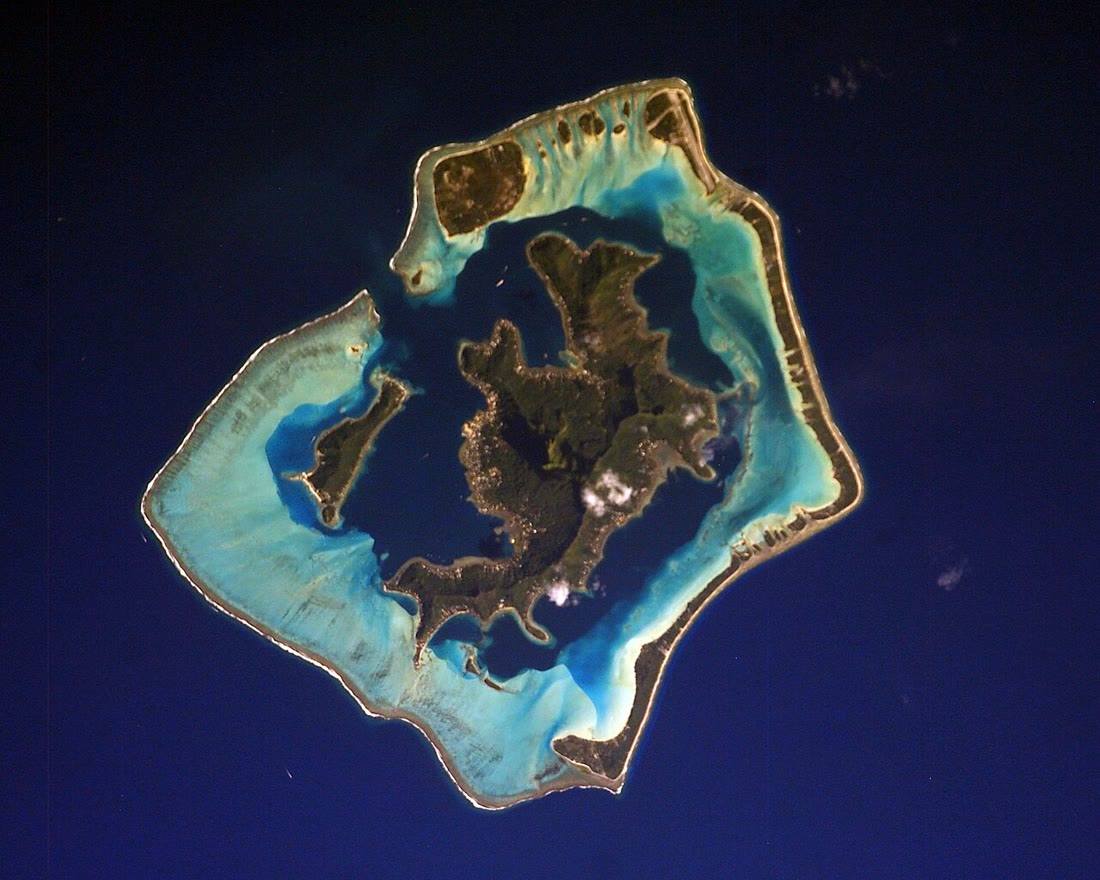
\includegraphics[height=6.9cm]{images/book3/b1-bora-bora.jpg}};
\end{tikzpicture}

{\small يسارًا: الأنواع الثلاثة \omterm{def:b1:chemical-biogenic-sediments:reef}{للشعاب المرجانية} في مقطع عرضي (تخطيطي، والمقياس الرأسي مبالغ فيه كثيرًا)، كما رسمها داروين: (أ)~شعاب هدبية تحيط بجزيرة بركانية؛ (ب)~غاصت الجزيرة، فصارت الشعاب، وهي تنمو نحو الأعلى، حاجزًا مفصولًا عن الشاطئ ببحيرة؛ (ج)~غاصت الجزيرة عن الأنظار، فالشعاب حلقة مرجانية حول بحيرة قاعها رسوب كربوناتي. ويمينًا: بورا بورا، جزيرة بركانية في بحيرة تحيط بها شعاب حاجزية، عليها جزر منخفضة، التقطها رائد فضاء من محطة الفضاء الدولية في 19 مارس 2003 (NASA, ملك عام، عبر Wikimedia Commons).}
\label{fig:b1:chemical-biogenic-sediments:reefs}
\end{omfigure}
% ledger: darwin:reefs, commons:bora-bora

\begin{history}[الشعاب على أسس تغوص، 1837--1842]
في أثناء رحلة السفينة \emph{بيغل}، أبحر تشارلز داروين بين شعاب المحيطين الهادئ والهندي. واستدلّ من حقيقة واحدة: فالمرجانيات بانية الشعاب، كما خلص، لا تزدهر في الأحوال العادية أعمق من بين 20 و\num{30} قامة، أي نحو 37 إلى \qty{55}{m}. ومع ذلك فالشعاب الحاجزية والحلقات المرجانية ترتفع من ماء عميق، بعيدًا جدًّا عن هذا الحدّ. فأسسها، كما رأى، لا بدّ أنها غاصت، ببطء كافٍ لتبقى المرجانيات قممها على السطح بالنموّ نحو الأعلى: فالشعاب الهدبية التي تحيط بجزيرة بركانية تصير حاجزًا كلما غاصت الجزيرة داخلها، وتصير حلقة مرجانية حين تختفي الجزيرة. وقد عرض نظريّته أمام الجمعية الجيولوجية في لندن في 31 مايو 1837، ونشرها عام 1842 في كتاب \emph{The Structure and Distribution of Coral Reefs}، مع خريطة لجميع الشعاب في العالم مرتّبة في الأنواع الثلاثة. أما لماذا تغرق الجزر المحيطية، وإلى أيّ حدّ، فهذا مسألة تبريد الصفيحة تحتها، وهو موضوع المجلد الثاني.
\end{history}
% ledger: darwin:reefs

تبقى الشعاب الحيّة فقط إن بقيت قمّتها في المياه الضحلة التي يعيش فيها بناتها. ومستوى البحر يتغيّر، وقد يغوص الأساس؛ والمهم هو مجموعهما، أي الارتفاع النسبي لمستوى البحر.

\begin{proposition}[البقاء بالنموّ أو الغرق]\label{prop:b1:chemical-biogenic-sediments:keep-up}
لتكن قمّة الشعاب على عمق $D_0$ تحت مستوى البحر، وتنمو نحو الأعلى بالمعدّل $a$، بينما يرتفع مستوى البحر النسبي بالمعدّل $r$، وكلاهما ثابت. فعمق الماء فوق الشعاب بعد الزمن $t$ هو
\[
D(t) = D_0 + (r - a)\,t .
\]
إن كان $a \ge r$ بقيت الشعاب تُواكب البحر (وعندما يكون $a > r$ تبلغ قمّتها السطح، ومن ثمّ لا تنمو إلا جانبيًّا)؛ وإن كان $a < r$ تتأخّر، فإن كان بناتها لا يعيشون أعمق من $D_{\max}$، غرقت بعد الزمن $(D_{\max} - D_0)/(r - a)$.
\end{proposition}

\begin{proof}
قِس الارتفاعات نحو الأعلى من علامة ثابتة على الأساس. قمّة الشعاب عند $h_0 + a t$ وسطح البحر عند $s_0 + r t$، فعمق الماء فوق القمّة هو $D = (s_0 - h_0) + (r - a)t = D_0 + (r-a)t$. فإذا كان $a > r$ يبلغ $D$ الصفر عند $t = D_0/(a-r)$، ولا تستطيع الشعاب النموّ فوق البحر. وإذا كان $a < r$ ينمو $D$ خطّيًّا، ويبلغ $D_{\max}$ حين يكون $(r-a)t = D_{\max} -
D_0$.
\end{proof}

لا تموت الشعاب التي غمرتها المياه في الحال، لكن الضوء يخفت، ويتغيّر البناة، وتبطؤ المصانع، فالشعاب التي تبدأ بالتأخّر تتأخّر أكثر. والشعاب والمنصّات المغمورة، المغطّاة برسوبيات أعماق البحار، توجد على منحدرات كثير من الجزر المحيطية وفي السجلّ الصخري.

عبر ملايين السنين تبني المصانع المنصّات الكربوناتية، وهي أجسام سميكة من كربونات المياه الضحلة تنمو مع هبوط أسسها. ويتكرّر شكلان (انظر الشكل أدناه). فالرفّ \emph{المحاط بحافة} له سطح مسطّح، محميّ خلف حافة من الشعاب وضحول الأويدات عند حدّه، تكسر الأمواج؛ وخلفه بحيرة هادئة من طين كلسي، وأمامه منحدر شديد تتساقط عليه الكتل والحطام المنفصل عن الحافة نحو الحوض. أما \emph{المنحدر} فيهبط بانحدار رقيق جدًّا من الشاطئ إلى الحوض بلا أي حافة: ضحول الأويدات ومصاطب من الأصداف حيث تحرّك الأمواج القاع، ثم طبقات من حطام الأصداف تجرفها العواصف، ثم طين كلسي تحت مدى الأمواج. ويكبر الرفّ المحاط بالحافة أساسًا نحو الأعلى والخارج من حافته، بينما يكبر المنحدر بتحريك أحزمة رسوبه نحو الشاطئ أو البحر مع ارتفاع البحر أو انخفاضه.

\begin{omfigure}
\begin{tikzpicture}[font=\footnotesize, >={Stealth[length=4pt]}]
% (a) rimmed shelf and (b) ramp, schematic cross-sections
\begin{scope}
  \fill[omSea] (0,0.2) rectangle (7.2,2.0);
  \fill[lith limestone, draw=black!60] (0,0) -- (0,1.55) -- (4.3,1.55) -- (4.5,1.75) -- (4.9,1.75) -- (5.1,1.5) -- (6.4,0.35) -- (7.2,0.3) -- (7.2,0) -- cycle;
  \fill[lith reef limestone, draw=black!70] (4.3,1.55) -- (4.5,1.75) -- (4.9,1.75) -- (5.1,1.5) -- (4.8,1.05) -- (4.3,1.05) -- cycle;
  \draw[omSea!60!black] (0,2.0) -- (7.2,2.0);
  \node at (2.1,1.78) {بحيرة: طين كلسي};
  \node[anchor=south, align=center, font=\scriptsize] at (4.7,2.05) {حافة الشعاب و\\ ضحول الأويدات};
  \node[anchor=west, font=\scriptsize] at (5.6,1.2) {المنحدر: حطام};
  \node[font=\scriptsize] at (6.75,0.75) {الحوض};
  \node at (3.6,-0.35) {(أ) رفّ محاط بحافة};
\end{scope}
\begin{scope}[xshift=8.0cm]
  \fill[omSea] (0,0.2) rectangle (7.2,2.0);
  \fill[lith limestone, draw=black!60] (0,0) -- (0,1.85) -- (7.2,0.55) -- (7.2,0) -- cycle;
  \draw[omSea!60!black] (0,2.0) -- (7.2,2.0);
  \draw[densely dashed, black!50] (0,1.6) -- (7.2,1.6) node[pos=1, anchor=south east, font=\scriptsize, inner sep=1pt] {أمواج الطقس الهادئ تبلغ};
  \draw[densely dashed, black!50] (0,1.0) -- (7.2,1.0) node[pos=1, anchor=south east, font=\scriptsize, inner sep=1pt] {أمواج العواصف تبلغ};
  \node[anchor=south, font=\scriptsize] at (0.9,2.05) {ضحول الأويدات};
  \node[anchor=south, font=\scriptsize] at (3.4,2.05) {طبقات أصداف العواصف};
  \node[anchor=south, font=\scriptsize] at (6.1,2.05) {طين كلسي};
  \node at (3.6,-0.35) {(ب) المنحدر المتدرّج};
\end{scope}
\end{tikzpicture}

{\small شكلا \omterm{def:b1:chemical-biogenic-sediments:reef}{المنصّة الكربوناتية} (تخطيطي، والمنحدرات مبالغ فيها كثيرًا). (أ)~رفّ محاط بحافة: حافة من الشعاب وضحول الأويدات تكسر الأمواج، وخلفها بحيرة هادئة من طين كلسي، والحطام المنفصل عن الحافة يتساقط على المنحدر نحو الحوض. (ب)~منحدر يهبط برفق من الشاطئ إلى الحوض، ورسوبه مفروز بحسب العمق الذي تصل إليه الأمواج.}
\label{fig:b1:chemical-biogenic-sediments:platforms}
\end{omfigure}

\section{الرسوبيات البيلاجية وعمق التعويض الكربوناتي}\label{sec:b1:chemical-biogenic-sediments:oozes}

بعيدًا عن اليابسة، لا يتلقّى قاع البحر من القارات إلا أدقّ الغبار الذي تحمله الرياح. وما يتساقط عليه بدلًا من ذلك هو هياكل العوالق التي عاشت في الماء المشمس على بُعد كيلومترات فوقه: الصفائح الكالسيتية للكوكوليتوفورات وأصداف الفورامينيفيرا، وأغلفة الدياتومات السيليسية المصنوعة من الأوبال، وهياكل الراديولاريا (يُعرض تصويرها بعد قليل). وهذا المطر الطويل من الكوكوليتات إلى قاع البحر هو العملية الرئيسية التي تصنع الطباشير ومعظم الحجر الكلسي في العالم.
% ledger: nasa:coccoliths-b3, og:carbonates

\begin{definition}[الرسوب الكلسي الناعم، والرسوب السيليسي الناعم]\label{def:b1:chemical-biogenic-sediments:ooze}
الرسوب الحيوي الناعم رسوب بيلاجي ناعم الحبيبات، يترسّب في المحيط المفتوح، ومكوّن في معظمه من هياكل العوالق. ويكون \emph{رسوبًا كلسيًّا ناعمًا}\index{رسوب كلسي ناعم} إذا كانت هياكله من كربونات الكالسيوم، وأهمّها الكوكوليتات والفورامينيفيرا، ويكون \emph{رسوبًا سيليسيًّا ناعمًا}\index{رسوب سيليسي ناعم} إذا كانت من الأوبال، أي السيليكا المائية غير المتبلورة، وأهمّها الدياتومات والراديولاريا.
\end{definition}
% ledger: og:carbonates

تغطّي الرسوبات الكلسية الناعمة نحو نصف قاع البحر في العالم، لكن فوق عمق معيّن فقط: فتختفي تحت نحو \qty{4500}{m}. والهياكل لا تكفّ عن السقوط هناك، بل تذوب. والمحيط العميق بارد والضغط عالٍ، وانحلالية الكالسيت تزداد مع العمق، بسبب الضغط أساسًا، بينما يقلّ تركيز أيون الكربونات في الماء عمومًا مع العمق (كيمياء هذه التوازنات مستعادة من كتب الكيمياء). وتحت عمق معيّن يكون الماء العميق غير مشبع بالكالسيت، والهياكل التي تصل إلى القاع تذوب أسرع كلما كانت أعمق.
% ledger: britannica:ccd, slotnick:ccd-definitions

\begin{omfigure}
\begin{tikzpicture}
\node[inner sep=0] (a) at (0,0) {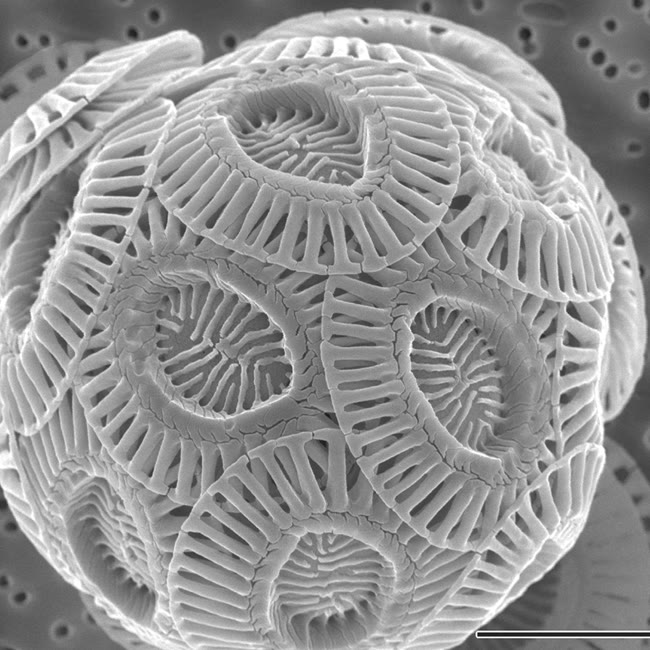
\includegraphics[height=4.3cm]{images/book3/b1-coccolithophore.jpg}};
\node[inner sep=0, anchor=west] (b) at ([xshift=0.25cm]a.east) {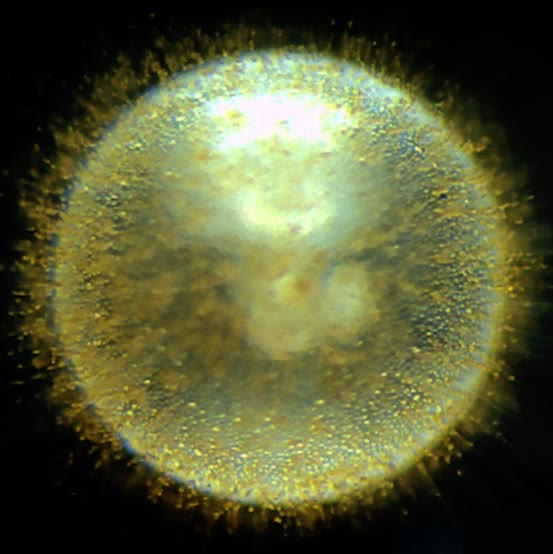
\includegraphics[height=4.3cm]{images/book3/b1-orbulina.jpg}};
\node[inner sep=0, anchor=west] (c) at ([xshift=0.25cm]b.east) {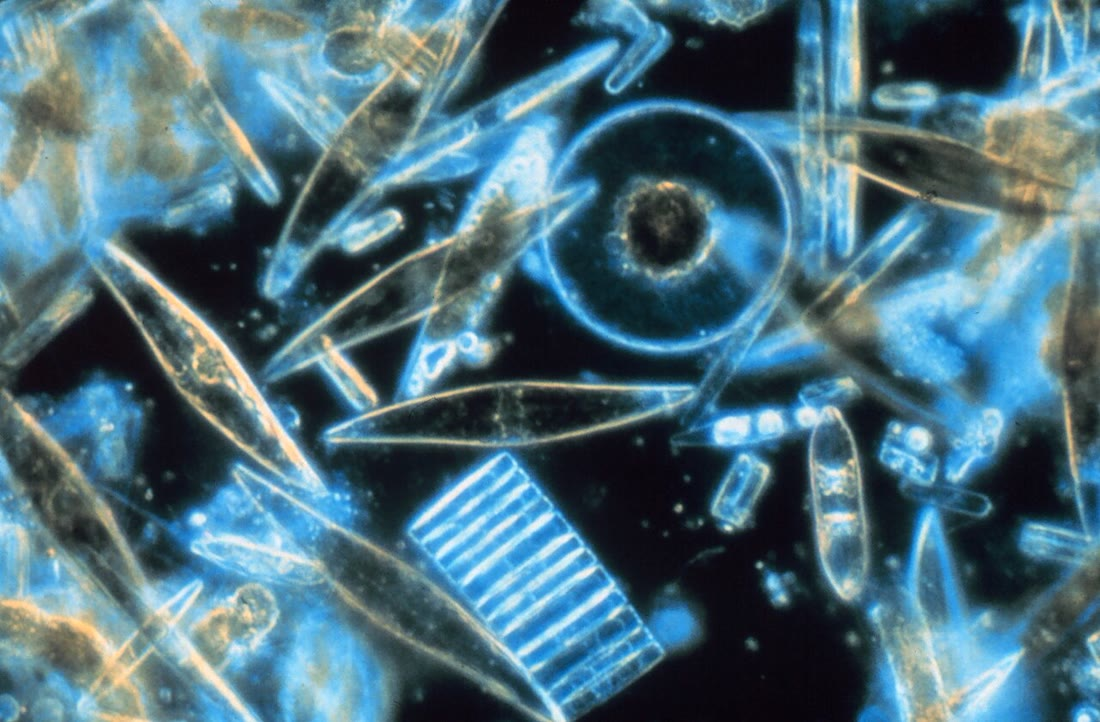
\includegraphics[height=4.3cm]{images/book3/b1-diatoms.jpg}};
\node[font=\footnotesize, anchor=north] at (a.south) {(أ) كوكوليتوفور};
\node[font=\footnotesize, anchor=north] at (b.south) {(ب) فورامينيفر};
\node[font=\footnotesize, anchor=north] at (c.south) {(ج) دياتومات};
\end{tikzpicture}

{\small صانعو الرسوبات الحيوية الناعمة. (أ)~خليّة واحدة من \emph{Emiliania huxleyi} مدرّعة بالكوكوليتات، صفائحها من الكالسيت (مجهر إلكتروني ماسح؛ Alison R.~Taylor, University of North Carolina Wilmington, CC~BY~2.5, عبر Wikimedia Commons). (ب)~فورامينيفر عوّامي حيّ، \emph{Orbulina universa}، صدفته الكالسيتية محاطة بأشواك (مجهر ضوئي؛ H.~Takagi and co-authors, 2019, CC~BY~4.0, عبر Wikimedia Commons). (ج)~دياتومات حيّة من الجليد البحري في مضيق ماكموردو بالقارة القطبية الجنوبية، كلّ منها في غلافه من الأوبال (مجهر ضوئي؛ Gordon T.~Taylor, Stony Brook University, NOAA, ملك عام، عبر Wikimedia Commons).}
\label{fig:b1:chemical-biogenic-sediments:plankton}
\end{omfigure}
% ledger: commons:ehux, commons:orbulina, commons:diatoms-noaa

\begin{definition}[الحدّ الانحلالي، وعمق التعويض الكربوناتي]\label{def:b1:chemical-biogenic-sediments:ccd}
\emph{الحدّ الانحلالي}\index{الحدّ الانحلالي} هو العمق في المحيط الذي يبدأ دونه انحلال الكالسيت على قاع البحر ظاهرًا في الرسوب، ويزداد معدّله بحدّة. و\emph{عمق التعويض الكربوناتي}\index{عمق التعويض الكربوناتي} (CCD) هو العمق الذي يتساوى عنده معدّل انحلال الكالسيت مع معدّل تساقط الكالسيت على قاع البحر؛ وتحته لا تتراكم كربونات الكالسيوم أبدًا. وعمليًّا يُحدَّد حيث يهبط محتوى كربونات الكالسيوم في الرسوب السطحي دون \qty{10}{\%} بالوزن.
\end{definition}
% ledger: slotnick:ccd-definitions

يقع التعويض الكربوناتي عمومًا على بُعد مئات الأمتار تحت \omterm{def:b1:chemical-biogenic-sediments:ccd}{الحدّ الانحلالي}. وليس مستوى ثابتًا: إذ تحدّده موازنة بين الإمداد والانحلال، فيقع أعمق حيث ينتج العوالق كربونات أكثر، وحيث يكون الماء العميق أقلّ تآكلًا. ففي الأطلسي يقع نحو \qty{500}{m} أعمق منه في المحيط الهادئ، نتيجة إمداد أعلى بالكربونات وانحلال أبطأ معًا؛ وفي غرب المحيط الهادئ وحده يقع نحو \qty{4000}{m} في الشمال الغربي، ونحو \qty{5100}{m} في وسط المحيط الهادئ. والأراغونيت، وهو أكثر ذوبانًا من الكالسيت، ينحلّ على أعماق أقلّ من ذلك. وعلى مدى الزمن الجيولوجي حرّكت تغيّرات الإمداد والإنتاجية والانحلال التعويض الكربوناتي بأكثر من \qty{2000}{m}.
% ledger: slotnick:ccd-definitions, britannica:ccd, zhang:ccd-west-pacific

\begin{method}[تحديد الحدّ الانحلالي والتعويض الكربوناتي]\label{met:b1:chemical-biogenic-sediments:ccd}
\begin{enumerate}
  \item اجمع أعلى بضعة سنتيمترات من الرسوب عند مواقع بأعماق مختلفة في منطقة واحدة، بعيدة بما يكفي عن اليابسة والتصاعد الصاعد، حتى يكون تخفيف الطين أو السيليس صغيرًا.
  \item قِس النسبة المئوية بالوزن ل\ce{CaCO3} في كل عيّنة، وارسمها بدلالة عمق الماء.
  \item \omterm{def:b1:chemical-biogenic-sediments:ccd}{الحدّ الانحلالي} هو العمق الذي يبدأ عنده المحتوى بالهبوط الحادّ، وحيث تُظهر الأصداف أولى علامات الانحلال (فورامينيفيرا مكسورة ومحفورة).
  \item التعويض الكربوناتي هو العمق الذي يهبط عنده المحتوى إلى \qty{10}{\%}: اقرأه بالاستيفاء الخطّي بين العينتين المحيطتين به على الجانبين.
\end{enumerate}
\end{method}

على جانب حيد محيطي، يكون قاع البحر فتيًّا وضحلًا قرب المحور، ويهبط مع تقدّم عمره وابتعاده عن المحور. وقطعة القاع التي وُلدت فوق التعويض الكربوناتي تجمع \omterm{def:b1:chemical-biogenic-sediments:ooze}{الرسوب الكلسي الناعم} حتى تهبط تحته؛ ومنذ ذلك الحين لا تتلقّى إلا ما لا ينحلّ: الغبار الذي يتساقط من الهواء فوقها، وأكاسيد الحديد والمنغنيز، وأسنان الأسماك. وهذا الرسوب البطيء البنّي هو الطين الأحمر في الأحواض العميقة.

\begin{proposition}[عبور التعويض الكربوناتي]\label{prop:b1:chemical-biogenic-sediments:flank}
ليكن قاع البحر بعمر $t$ على العمق $d(t) = d_r + C\sqrt t$ (\cref{thm:b1:rifts-ridges-margins:depth-age})، ومحور الحيد على العمق $d_r$، وهو أقلّ عمقًا من \omterm{def:b1:chemical-biogenic-sediments:ccd}{عمق التعويض الكربوناتي} $z_c$ الثابت. فيمرّ القاع تحت التعويض الكربوناتي عند العمر
\[
t_c = \left(\frac{z_c - d_r}{C}\right)^2 ,
\]
ويحمل موقعٌ عمره $t > t_c$ من الأسفل إلى الأعلى \omterm{def:b1:layered-earth:layers}{القشرة} البركانية، \omterm{def:b1:chemical-biogenic-sediments:ooze}{والرسوب الكلسي الناعم} المترسّب خلال الزمن $t_c$، والطين الأحمر المترسّب خلال الزمن $t - t_c$.
\end{proposition}

\begin{proof}
يزداد العمق $d(t)$ مع $t$، و$d(t_c) = z_c$ يعطي $C\sqrt{t_c} =
z_c - d_r$، ومنه $t_c$. فقبل $t_c$ يكون القاع فوق التعويض الكربوناتي، حيث يتساقط الكالسيت أسرع مما ينحلّ ويتجمّع الرسوب الناعم؛ وبعد $t_c$ يكون تحته، حيث لا تتراكم كربونات، ولا يُضاف إلا الطين غير القابل للانحلال. والرسوب الناعم، بعدما يُدفن تحت الطين، يُحمى من الماء المآكل فوقه، فترتيب الطبقات هو ترتيب الأزمنة.
\end{proof}

مع $d = 2500 + 350\sqrt t$ (بالمتر، و$t$ بالملايين من السنين)، يعبر \omterm{def:b1:isostasy-gravity:isostasy}{عمق التعويض} \qty{4500}{m} عند العمر $(2000/350)^2 = \qty{32.7}{Myr}$؛ وبمعدّل انتشار نصفي قدره \qty{25}{mm} في السنة يكون ذلك على بُعد \qty{816}{km} من المحور (الشكل أدناه). ويعود هذا الترتيب نفسه مرة بعد مرة عند حفر قاع محيطي قديم: بازلت، ثم \omterm{def:b1:chemical-biogenic-sediments:ooze}{الرسوب الكلسي الناعم} أو الطباشير، ثم الطين الأحمر، سجلّ رحلة القاع نزولًا على المنحدر. وحيث تحرّكت الصفيحة بعد ذلك تحت حزام إنتاجية عالية، قرب خط الاستواء، يمكن أن يُغطّى الطين بطبقة جديدة من الرسوب الكلسي، وهكذا تسجّل اللُّبّات حركة الصفائح كما تسجّل \omterm{def:b1:chemical-biogenic-sediments:ccd}{عمق التعويض الكربوناتي}.
% ledger: parsons:plate-model

\begin{omfigure}
\begin{tikzpicture}[font=\footnotesize]
\begin{axis}[width=11cm, height=5.6cm, xmin=0, xmax=1750, ymin=2000, ymax=6200, y dir=reverse,
    xlabel={المسافة من محور الحيد (\unit{km})، معدّل الانتشار النصفي \qty{25}{mm.yr^{-1}}},
    ylabel={العمق (m)}, ytick={2000,3000,...,6000},
    axis on top, clip=false]
  % sea water above the floor
  \addplot[fill=omSea, draw=none] table[x=x_km, y=depth] {figdata/out/bachelor-1-ccd_flank-profile.dat} -- (axis cs:1750,2000) -- (axis cs:0,2000) -- cycle;
  % floor: ooze-covered above the CCD, red clay below
  \addplot[very thick, draw=omLithLime!70!black, restrict x to domain=0:816.3] table[x=x_km, y=depth] {figdata/out/bachelor-1-ccd_flank-profile.dat};
  \addplot[very thick, draw=brown!70!black, restrict x to domain=816.3:1750] table[x=x_km, y=depth] {figdata/out/bachelor-1-ccd_flank-profile.dat};
  \draw[thick, omThm, densely dashed] (axis cs:0,4500) -- (axis cs:1750,4500) node[pos=0.99, anchor=north east, inner sep=1.5pt] {CCD, \qty{4500}{m}};
  \draw[black!60, dotted, thick] (axis cs:0,4050) -- (axis cs:1750,4050) node[pos=0.99, anchor=south east, inner sep=1.5pt] {الحدّ الانحلالي (تخطيطي)};
  \fill[omThm] (axis cs:816.3,4500) circle[radius=2pt];
  \node[anchor=north east, align=right] at (axis cs:790,4620) {القاع يعبر التعويض الكربوناتي\\ عند \qty{32.7}{Myr}، \qty{816}{km}};
  \node[anchor=north, align=center, omLithLime!40!black] at (axis cs:520,2750) {رسوب كلسي ناعم\\ يتراكم};
  \node[anchor=north west, align=left, brown!60!black] at (axis cs:1000,5180) {طين أحمر فوق\\ رسوب مدفون};
\end{axis}
% sediment column at the site 1500 km from the axis (60 Myr), schematic
\begin{scope}[xshift=10.6cm, yshift=0.4cm]
  \draw[lith basalt] (0,0) rectangle (0.9,1.0);
  \draw[lith limestone] (0,1.0) rectangle (0.9,2.6);
  \fill[brown!45, draw=black!60] (0,2.6) rectangle (0.9,3.2);
  \node[anchor=west, align=left, font=\scriptsize] at (1.0,0.5) {قشرة بازلتية};
  \node[anchor=west, align=left, font=\scriptsize] at (1.0,1.8) {رسوب كلسي ناعم\\ (من 0 إلى \qty{32.7}{Myr})};
  \node[anchor=west, align=left, font=\scriptsize] at (1.0,2.9) {طين أحمر};
  \node[anchor=south, font=\scriptsize, align=center] at (0.9,3.3) {عمود عند \qty{1500}{km}\\ (تخطيطي)};
\end{scope}
\end{tikzpicture}

{\small رواسب بيلاجية على جانب حيد. يعمق القاع مع العمر وفق \omterm{thm:b1:rifts-ridges-margins:depth-age}{قانون العمق–العمر} $d = 2500 + 350\sqrt t$، ويبتعد عن المحور بمعدّل \qty{25}{mm} في السنة؛ فوق \omterm{def:b1:chemical-biogenic-sediments:ccd}{عمق التعويض الكربوناتي}، المأخوذ هنا \qty{4500}{m}، يتجمّع \omterm{def:b1:chemical-biogenic-sediments:ooze}{رسوب كلسي ناعم}، وتحته لا يوجد إلا الطين الأحمر. وموقع بعيد عن المحور يحمل البازلت والرسوب الكلسي والطين الأحمر، من الأسفل إلى الأعلى (العمود على اليمين، والسماكات تخطيطية). \omterm{def:b1:chemical-biogenic-sediments:ccd}{والحدّ الانحلالي}، المرسوم على بُعد بضع مئات من الأمتار فوق التعويض الكربوناتي، يبيّن حيث يبدأ الانحلال في الظهور.}
\label{fig:b1:chemical-biogenic-sediments:flank}
\end{omfigure}
% computed in figdata/bachelor-1/ccd_flank.py; ledger: parsons:plate-model, britannica:ccd, slotnick:ccd-definitions

\section{الرسوبات السيليسية والصوّان}\label{sec:b1:chemical-biogenic-sediments:silica}

الدياتومات، وهي طحالب وحيدة الخلية من العوالق، والراديولاريا، وهي أعضاء وحيدة الخلية من حيوانات العوالق، تبني هياكلها من الأوبال، تأخذه من حمض السيليسيك المذاب في ماء البحر. وخلافًا لكالسيت المحيط السطحي، لا يحميه الإشباع الفائق: فماء البحر غير مشبع به في كل الأعماق، ومعظم الأوبال يذوب ما إن يموت الكائن، أولًا في الماء وهو يهبط ثم على قاع البحر. ومن 255 تيرامول من السيليكون التي تبنيها عوالق المحيط العالمي في الأوبال كل سنة، لا يُدفن منها في الرسوب نهائيًّا إلا نحو 9.2: أي حفظ بنسبة \qty{3.6}{\%}. وذرّة السيليكون التي يجلبها نهر إلى البحر تأخذها العوالق وتطلقها من جديد نحو ست عشرة مرّة قبل أن تُدفن، وتبقى نحو \num{8000} سنة في المحيط.
% ledger: treguer:silica

ولهذا تتكوّن الرسوبات السيليسية الناعمة حيث يكون إنتاج الأوبال عاليًا جدًّا، حتى تتراكم نسبة \qty{3.6}{\%} منه، وحيث لا يخفّفه شيء آخر تقريبًا: حول المحيط الجنوبي، وفي شمال المحيط الهادئ، وعلى طول خطّ الاستواء في المحيط الهادئ، وعلى الهوامش القارية، أي حيث يصعد الماء العميق الغنيّ بالمغذّيات إلى السطح (\cref{ch:b1:ocean-circulation}). وتهيمن أيضًا تحت التعويض الكربوناتي تحت المياه الخصبة، حيث انحلّت الكالسيتات التي تساقطت معها.
% ledger: treguer:silica, og:carbonates

\begin{definition}[الصوّان]\label{def:b1:chemical-biogenic-sediments:chert}
\emph{الصوّان}\index{الصوّان} صخر رسوبي صلب كثيف من كوارتز دقيق التبلّر، يتكوّن في أغلب الحالات من أوبال حيوي ذاب وأعيد تبلّره بعد الدفن؛ ويوجد في طبقات، غالبًا من الرسوبات السيليسية الناعمة، أو في عُقَد، وأشهرها عُقَد الصوّان في الطباشير.
\end{definition}
% ledger: og:carbonates

أما رسوب الدياتومات الذي لم يُعَد تبلّره فيصير الدياتوميت، صخرًا خفيفًا أبيض مسامّيًّا، يكاد يكون أوبالًا نقيًّا. ومع الدفن والزمن يتحوّل الأوبال إلى أشكال أخرى من السيليكا، وأخيرًا إلى كوارتز، وتهاجر السيليكا: فتخرج من الطباشير مثلًا، وتتجمّع في عُقَد من \omterm{def:b1:chemical-biogenic-sediments:chert}{الصوّان} على طول طبقات معيّنة. وكيف يحدث ذلك يعود إلى علم الدياجينيز (\cref{ch:b1:diagenesis-basins}).

\section{الرسوبات التبخّرية}\label{sec:b1:chemical-biogenic-sediments:evaporites}

حيث يفقد جسم من ماء البحر بالتبخّر ماءً أكثر مما يتلقّى، تتركّز أملاحه حتى تترسّب واحدًا بعد الآخر. وتركيب ماء البحر هو نفسه، في أيوناته الرئيسية، في كل المحيطات (\cref{tab:b1:chemical-biogenic-sediments:seawater}).

\begin{table}[htbp]
\centering\small
\begin{tabular}{@{}lrrr@{}}
\hline
الأيون & الكسر الكتلي من ملح البحر & \si{g} لكل \si{kg} من ماء البحر & \si{mmol} لكل \si{kg} \\
\hline
كلوريد \ce{Cl-} & 0.5503 & 19.353 & 545.9 \\
صوديوم \ce{Na+} & 0.3066 & 10.781 & 469.0 \\
كبريتات \ce{SO4^2-} & 0.0771 & 2.712 & 28.2 \\
ماغنيسيوم \ce{Mg^2+} & 0.0365 & 1.284 & 52.8 \\
كالسيوم \ce{Ca^2+} & 0.0117 & 0.412 & 10.3 \\
بوتاسيوم \ce{K+} & 0.0113 & 0.399 & 10.2 \\
بيكربونات الهيدروجين \ce{HCO3-} & 0.0030 & 0.105 & 1.72 \\
بروميد \ce{Br-} & 0.0019 & 0.067 & 0.84 \\
\hline
كل المذابات & 1 & 35.165 & \\
\hline
\end{tabular}
\caption{الأيونات الرئيسية لماء البحر بالتركيب المرجعي، عند ملوحة \qty{35.165}{g} من الملح لكل كيلوغرام من ماء البحر. يكوّن الكلوريد والصوديوم \qty{86}{\%} من الملح بالكتلة؛ أما معظم الباقي فالكربونات والسترونتيوم والبورات والفلوريد.}
\label{tab:b1:chemical-biogenic-sediments:seawater}
\end{table}
% ledger: teos10:reference-composition, teos10:reference-salinity (g and mmol computed in evaporation.py)

\begin{definition}[الرسوب التبخّري، وتتابع التبخّر، والسبخة]\label{def:b1:chemical-biogenic-sediments:evaporite}
\emph{الرسوب التبخّري}\index{الرسوب التبخّري} هو رسوب أو صخر رسوبي من أملاح ترسّبت من محلول ملحي طبيعي تركّز بالتبخّر: أساسًا الجبس \ce{CaSO4.2H2O} والأنهيدريت \ce{CaSO4}، والهاليت \ce{NaCl}، وأملاح البوتاسيوم والماغنيسيوم. و\emph{تتابع التبخّر}\index{تتابع التبخّر} هو الترتيب الذي تترسّب به \omterm{def:b1:rock-forming-minerals:mineral}{المعادن} من ماء البحر المتبخّر، وأقلّها ذوبانًا أولًا: كربونات الكالسيوم، ثم الجبس، ثم الهاليت، ثم أملاح البوتاسيوم والماغنيسيوم. و\emph{السبخة}\index{السبخة} سهل ملحي ساحلي، عند مستوى أعلى المدّات أو فوقه بقليل، تنمو فيه الجبس والأنهيدريت والهاليت داخل الرسوب من الماء المالح المتبخّر الذي يتشرّبه.
\end{definition}
% ledger: og:carbonates, warren:brine-stages

رصد أوسيليو هذا التتابع منذ عام 1849، حين بخّر وعاءً من ماء البحر حتى الجفاف؛ وأدقّ القياسات تأتي من أملاح جزيرة إيناغوا الكبرى في جزر البهاما، حيث يُقاد ماء البحر عبر سلسلة أحواض متزايدة التركيز. وتبدأ كربونات الكالسيوم بالترسّب حين يصير المحلول الملحي أكثر تركيزًا من ماء البحر ب\num{1.8} مرة، والجبس عند 3.8 مرة، والهاليت عند 10.6 مرة؛ وفي المختبر تلتها كبريتات الماغنيسيوم عند نحو 70 مرة، وأملاح البوتاسيوم فوق 90 مرة. وبما أن الأملاح التي تترسّب قبلها جزء ضئيل من الكتلة، فإن معامل التركيز 10.6 يعني أن $1/10.6$، أي نحو \qty{9}{\%}، من الماء يبقى: فالهاليت لا يأتي إلا بعد أن تذهب تسعة أعشار الماء (الشكل أدناه، اللوحة~أ). ويزداد المحلول الملحي كثافةً كلما تركّز، من \qty{1.03}{g.cm^{-3}} لماء البحر إلى نحو \num{1.13} عند تكوّن الجبس، و\num{1.22} مع الهاليت، وأكثر من \num{1.30} مع أملاح المرّ، وهي آخر الأملاح جميعها.
% ledger: warren:brine-stages, mccaffrey:thresholds

وكم يعطي كيلوغرام من ماء البحر من كل ملح يُحسب من \cref{tab:b1:chemical-biogenic-sediments:seawater} بعدّ الأيون الذي ينفد أولًا. فكربونات الكالسيوم يحدّها الكربونات وبيكربونات الهيدروجين، أي \qty{1.10}{mmol}، نحو \qty{0.11}{g}. ويأخذ الجبس الكالسيوم المتبقّي، أي \qty{9.18}{mmol}، أي \qty{1.58}{g}، والكبريتات فائضة. ويأخذ الهاليت كل الصوديوم، أي \qty{469}{mmol}، أي \qty{27.4}{g}، والكلوريد فائض. وما يبقى، نحو \qty{6.3}{g} من الماغنيسيوم والبوتاسيوم والكبريتات والكلوريد والبروميد، يكوّن أملاح المرّ. والهاليت يمثّل \qty{78}{\%} من المجموع: فحوض تبخّري جفّ هو قبل كل شيء كتلة من ملح الصخر.
% computed in figdata/bachelor-1/evaporation.py; ledger: teos10:reference-composition, mccaffrey:thresholds

\begin{omfigure}
\begin{tikzpicture}[font=\footnotesize]
\begin{axis}[name=a, width=7.6cm, height=5.6cm, xmode=log, xmin=1, xmax=100, ymin=0, ymax=1.05,
    xlabel={معامل تركّز المحلول الملحي}, ylabel={كسر الماء المتبقّي},
    title={\footnotesize (أ) بدايات تتابع التبخّر}, grid=major, grid style={black!10},
    log ticks with fixed point]
  \addplot[omDef, thick] table[x=CF, y=f_left] {figdata/out/bachelor-1-evaporation-curve.dat};
  \addplot[omThm, only marks, mark=*, mark size=1.8pt] table[x=CF, y=f_left] {figdata/out/bachelor-1-evaporation-steps.dat};
  \node[anchor=south west, font=\scriptsize] at (axis cs:1.8,0.556) {\ce{CaCO3} (1.8)};
  \node[anchor=south west, font=\scriptsize] at (axis cs:3.8,0.263) {الجبس (3.8)};
  \node[anchor=south west, font=\scriptsize] at (axis cs:10.6,0.094) {الهاليت (10.6)};
  \node[anchor=south, font=\scriptsize, align=center] at (axis cs:60,0.16) {أملاح Mg وK\\ (70, 90)};
\end{axis}
\begin{axis}[at={(a.east)}, anchor=west, xshift=1.7cm, width=7.0cm, height=5.6cm,
    ybar, bar width=14pt, ymin=0, ymax=32, xmin=0.4, xmax=4.6,
    xtick={1,2,3,4}, xticklabels={{\ce{CaCO3}}, {الجبس}, {الهاليت}, {أملاح المرّ}},
    ylabel={غرامات لكل كيلوغرام من ماء البحر}, title={\footnotesize (ب) الكتل المترسّبة},
    nodes near coords, nodes near coords style={font=\scriptsize, /pgf/number format/precision=2},
    every node near coord/.append style={/pgf/number format/fixed}]
  \addplot[fill=omDef!40, draw=omDef] table[x=idx, y=g_per_kg] {figdata/out/bachelor-1-evaporation-masses.dat};
\end{axis}
\end{tikzpicture}

{\small تبخّر ماء البحر. (أ)~كسر الماء المتبقّي عندما يتركّز المحلول الملحي بمعامل معيّن، مع بداية كل \omterm{def:b1:rock-forming-minerals:mineral}{معدن} كما قيست في أحواض إيناغوا الكبرى وفي المختبر (McCaffrey, Lazar and Holland, 1987). (ب)~الكتل المترسّبة لكل كيلوغرام من ماء البحر المبخّر حتى الجفاف، إذ يأخذ كل \omterm{def:b1:rock-forming-minerals:mineral}{معدن} كل الأيون الذي يحدّه (الجبس محسوب مع مائه، وأملاح المرّ دون مائها)، محسوبةً من التركيب المرجعي لماء البحر.}
\label{fig:b1:chemical-biogenic-sediments:evaporation}
\end{omfigure}
% computed in figdata/bachelor-1/evaporation.py; ledger: mccaffrey:thresholds, teos10:reference-composition

ومن هذه الكتل تتبع سماكة الملح الذي يمكن لجسم ماء معيّن أن يتركه مباشرة.

\begin{proposition}[ملح من عمود من ماء البحر]\label{prop:b1:chemical-biogenic-sediments:column}
عمود من ماء البحر ارتفاعه $H$ وكثافته $\rho_{sw}$، يُبخَّر حتى الجفاف، فيضع طبقة من \omterm{def:b1:rock-forming-minerals:mineral}{معدن} كثافته $\rho_x$، سمكها
\[
h_x = \frac{\rho_{sw}\,H\,m_x}{\rho_x},
\]
حيث $m_x$ كتلة ذلك \omterm{def:b1:rock-forming-minerals:mineral}{المعدن} المترسّبة لكل وحدة كتلة من ماء البحر.
\end{proposition}

\begin{proof}
تحمل وحدة المساحة من العمود كتلة $\rho_{sw}H$ من ماء البحر، يترسّب منها كتلة $\rho_{sw}Hm_x$ من \omterm{def:b1:rock-forming-minerals:mineral}{المعدن}. وموزّعةً على وحدة المساحة نفسها كطبقة كثافتها $\rho_x$، يكون سمكها $\rho_{sw}Hm_x/\rho_x$.
\end{proof}

ب$\rho_{sw} = \qty{1030}{kg.m^{-3}}$، و$m = \qty{27.4}{g.kg^{-1}}$، وكثافة الهاليت \qty{2170}{kg.m^{-3}}، يترك عمود من ماء البحر ارتفاعه \qty{1000}{m} طبقة من الهاليت سمكها \qty{13.0}{m}؛ ومع الجبس، كثافته \qty{2300}{kg.m^{-3}}، يترك \qty{0.71}{m} من الجبس. وهذه هي مشكلة السماكة في \omterm{def:b1:chemical-biogenic-sediments:evaporite}{الرسوبات التبخّرية}: فطبقات الملح التي تبلغ مئات الأمتار أو كيلومترات في السماكة لا يمكن أن تكون بقايا ملء واحد لأيّ حوض، مهما كان عميقًا.
% computed in figdata/bachelor-1/evaporation.py; ledger: warren:brine-stages, webmineral:evaporites

والجواب حوض يستمرّ في تلقّي ماء البحر. فحوض مفصول عن المحيط بعتبة، أو مضيق ضحل، أو حاجز، في مناخ جاف، يفقد الماء بالتبخّر على كامل مساحته؛ فيتدفّق ماء البحر فوق العتبة ليعوّضه، جالبًا ملحًا جديدًا، ويمكن للمحلول الملحي الأثقل أن يتدفّق خارجًا في العمق فوق العتبة (الشكل أدناه). وتركيز المحلول الملحي يحدّده توازن هذه التدفّقات.

\begin{proposition}[الحوض المحجوز]\label{prop:b1:chemical-biogenic-sediments:barred}
ليفقد حوض جيّد الخلط مساحته $A$ حجم $EA$ من الماء في وحدة الزمن بالتبخّر الصافي، ويتلقّى ماء بحر بمعدّل حجمي $Q_{\mathrm{in}}$، ويعيد المحلول الملحي إلى المحيط بمعدّل حجمي $Q_{\mathrm{out}}$، في حالة مستقرّة. وبالنسبة إلى أيون لا يترسّب، يتركّز المحلول الملحي بالمعامل
\[
k = \frac{Q_{\mathrm{in}}}{Q_{\mathrm{out}}} = \frac{Q_{\mathrm{in}}}{Q_{\mathrm{in}} - EA}
\]
بالنسبة إلى ماء البحر (الحجوم محسوبة كأنها بكثافة متساوية).
\end{proposition}

\begin{proof}
في الحالة المستقرّة لا يتغيّر حجم الحوض، فيتعادل الداخل مع الخارج والتبخّر: $Q_{\mathrm{in}} = Q_{\mathrm{out}} +
EA$. يدخل الأيون بتركيز $c_0$ لماء البحر، ولا يخرج إلا مع المحلول الملحي بتركيزه $c$؛ وبما أنه لا يترسّب، فإن كتلته في الحوض تبقى ثابتة حين يكون $Q_{\mathrm{in}}c_0 = Q_{\mathrm{out}}c$. ومنه $c/c_0 =
Q_{\mathrm{in}}/Q_{\mathrm{out}}$، وبتعويض $Q_{\mathrm{out}}$ نحصل على الصيغة الثانية.
\end{proof}

يتحكّم الخارج فيما يرسّبه الحوض. فإن عاد أكثر من عُشر الداخل إلى المحيط محلولًا ملحيًّا، بقي $k$ أدنى من 10.6، ورسّب الحوض الكربونات والجبس دون الهاليت أبدًا؛ وإن كان الخارج أقلّ، بلغ المحلول الملحي تشبّع الهاليت، وامتلأ الحوض بالملح؛ وإن أُغلق المضيق تمامًا، جفّ الحوض وانخفض مستواه بمعدّل $E$.

\begin{omfigure}
\begin{tikzpicture}[font=\footnotesize, >={Stealth[length=4pt]}]
% barred evaporite basin (schematic)
\fill[omSea] (0,1.0) rectangle (3.2,3.0);
\fill[omSea!70!yellow!40] (3.6,0.6) rectangle (11.2,3.0);
\fill[omSea] (3.0,2.45) rectangle (3.8,3.0);
\draw[lith shale] (0,0) -- (0,1.0) -- (2.6,1.0) -- (3.2,2.4) -- (3.6,2.45) -- (4.4,0.6) -- (10.2,0.6) -- (11.2,2.2) -- (11.2,0) -- cycle;
\draw[lith evaporite] (4.25,0.95) -- (4.4,0.6) -- (10.2,0.6) -- (10.41,0.95) -- cycle;
\fill[omLithGranite!50, draw=black!50] (5.6,0.95) rectangle (9.0,1.35);
\draw[omSea!60!black] (0,3.0) -- (11.2,3.0);
\draw[->, thick, omDef] (1.6,2.75) -- (4.6,2.75) node[right] {تدفّق ماء البحر الداخل};
\draw[->, thick, omThm, densely dashed] (4.6,1.5) .. controls (4.1,2.35) and (3.8,2.57) .. (3.1,2.57) .. controls (2.6,2.57) and (2.3,2.2) .. (2.1,1.7) node[anchor=north east, inner sep=1pt] {تدفّق المحلول الملحي الخارج};
\foreach \x in {6.0,7.4,8.8,10.2} {\draw[->, black!60] (\x,3.1) -- (\x,3.7);}
\node[anchor=south] at (8.1,3.7) {تبخّر فوق الحوض};
\node at (0.8,2.15) {المحيط};
\node[anchor=south] at (3.4,3.0) {العتبة};
\node[anchor=north, fill=white, inner sep=1pt] at (7.3,0.55) {الجبس والأنهيدريت};
\node at (7.3,1.15) {الهاليت};
\node at (7.3,2.2) {محلول ملحي كثيف};
\end{tikzpicture}

{\small حوض تبخّري محجوز (تخطيطي): يتدفّق ماء البحر فوق عتبة ليعوّض الماء المتبخّر من الحوض؛ ينزل المحلول الكثيف، ويعود جزء منه إلى المحيط في العمق. وكلما قلّ الخارج زاد تركّز المحلول؛ وهنا جاوز تشبّع الهاليت، فيقع الهاليت فوق الجبس الأسبق.}
\label{fig:b1:chemical-biogenic-sediments:barred}
\end{omfigure}

أكبر \omterm{def:b1:chemical-biogenic-sediments:evaporite}{رسوب تبخّري} حديث في العالم يرقد تحت قاع البحر الأبيض المتوسط. وبين \num{5.97} و\num{5.33} مليون سنة مضت، في عصر المسينيان، كانت تبادلات الماء بين البحر المتوسط والأطلسي مقيّدة، وترسّبت في الأحواض العميقة تبخّريات يبلغ سمكها \qty{2}{km}، معظم هاليتها في فترة قصيرة بين \num{5.60} و\num{5.55} مليون سنة. وكيف حدث ذلك ما زال محلّ جدل. ففي نموذج منها كان البحر مقطوعًا إلى حدّ كبير، وانخفض مستواه بنحو \qty{1500}{m}، فصارت الأحواض العميقة بحيرات ملحية، وحفرت الأنهار أخاديد عميقة في الهوامش الجافّة؛ وفي نماذج أخرى ظلّ الحوض متصلًا وممتلئًا، حوضًا محجوزًا على نطاق واسع. وكلاهما يجب أن يفسّر كيلومترات من الملح، وهو ما كان ليعطيه ملء واحد للبحر أبدًا.
% ledger: vasiliev:msc

\section{التمارين}

\begin{exercise}[$\star$]\label{exo:b1:chemical-biogenic-sediments:1}
يحتوي ماء البحر ذو التركيب المرجعي على \qty{35.165}{g} من الملح لكل كيلوغرام، ومنه الكسور الكتلية للكلوريد والصوديوم والكبريتات والماغنيسيوم \num{0.5503} و\num{0.3066} و\num{0.0771} و\num{0.0365}. احسب كتلة كل أيون في كيلوغرام من ماء البحر، وكسر الملح المكوّن من الصوديوم والكلوريد معًا.
% ledger: teos10:reference-composition, teos10:reference-salinity
\end{exercise}

\begin{exercise}[$\star$]\label{exo:b1:chemical-biogenic-sediments:2}
يبدأ ترسّب كربونات الكالسيوم والجبس والهاليت وكبريتات الماغنيسيوم من ماء بحر مُركّز \num{1.8} و\num{3.8} و\num{10.6} و\num{70} مرة. احسب لكل منها كسر الماء المتبقّي والكسر الذي تبخّر.
% ledger: mccaffrey:thresholds
\end{exercise}

\begin{exercise}[$\star$]\label{exo:b1:chemical-biogenic-sediments:3}
على شعاب تهيمن عليها \emph{Acropora} تبلغ الميزانية الكربوناتية \qty{8.4}{kg} من \ce{CaCO3} لكل متر مربّع في السنة، وتنمو الشعاب بمقدار \qty{4.2}{mm} في السنة. (أ)~باستعمال \cref{prop:b1:chemical-biogenic-sediments:accretion}، احسب الكثافة الحجمية الجافّة للشعاب. (ب)~ما مساميّتها إن كانت حبيباتها أراغونيتًا، كثافته \qty{2.93}{g.cm^{-3}}؟ أم كالسيتًا، كثافته \qty{2.71}{g.cm^{-3}}؟ (ج)~عند الكثافة الحجمية نفسها، بأيّ سرعة تنمو شعاب ميزانيتها المتوسطة \qty{3.7}{kg.m^{-2}.yr^{-1}}؟
% ledger: perry:chagos, webmineral:polymorphs, hom:calcite
\end{exercise}

\begin{exercise}[$\star$]\label{exo:b1:chemical-biogenic-sediments:4}
تحتوي الرسوبات السطحية من منطقة في قاع البحر على النسب المئوية بالوزن التالية من \ce{CaCO3}: 88 عند \qty{3000}{m}، و\num{85} عند \qty{3500}{m}، و\num{80} عند \qty{4000}{m}، و\num{62} عند \qty{4300}{m}، و\num{35} عند \qty{4500}{m}، و\num{12} عند \qty{4700}{m}، و\num{6} عند \qty{4800}{m}، و\num{2} عند \qty{5000}{m}. باستعمال \cref{met:b1:chemical-biogenic-sediments:ccd}، حدّد \omterm{def:b1:chemical-biogenic-sediments:ccd}{الحدّ الانحلالي} والتعويض الكربوناتي.
\end{exercise}

\begin{exercise}[$\star\star$]\label{exo:b1:chemical-biogenic-sediments:5}
(أ)~اكتب معادلة التوازن لترسّب كربونات الكالسيوم من أيوني الكالسيوم وبيكربونات الهيدروجين، واحسب كتلة ثاني أكسيد الكربون المنطلق لكل كيلوغرام من \ce{CaCO3} المترسّب (الكتلتان المولاريتان \qty{100.09}{g.mol^{-1}} و\qty{44.01}{g.mol^{-1}}). (ب)~كم يطلق من ثاني أكسيد الكربون شعاب ميزانيتها \qty{3.7}{kg.m^{-2}.yr^{-1}} لكل متر مربّع في السنة، بحسب هذه المعادلة؟ (ج)~لماذا تطلق شعاب تحوّل الكربون المذاب إلى صخر ثاني أكسيد الكربون؟
% ledger: perry:chagos
\end{exercise}

\begin{exercise}[$\star\star$]\label{exo:b1:chemical-biogenic-sediments:6}
خذ قاع البحر على العمق $d = 2500 + 350\sqrt t$ (بالمتر، و$t$ بالملايين من السنين)، ينتشر من حيده بمعدّل نصفي \qty{25}{mm} في السنة. (أ)~في أيّ عمر وعلى أيّ بُعد من المحور يعبر تعويضًا كربوناتيًّا عند \qty{4500}{m}؟ (ب)~الأمر نفسه لتعويض عند \qty{5100}{m}، كما في وسط المحيط الهادئ. (ج)~كم كان قاع عمره \qty{60}{Myr} سيتلقّى من الطين الأحمر في كل حالة؟
% ledger: parsons:plate-model, zhang:ccd-west-pacific
\end{exercise}

\begin{exercise}[$\star\star$]\label{exo:b1:chemical-biogenic-sediments:7}
شعبة مرجانية تنمو بمقدار \qty{4.2}{mm} في السنة. (أ)~هل تستطيع مواكبة ارتفاع نسبي لمستوى البحر قدره \qty{3}{mm} في السنة؟ (ب)~قمّتها على عمق \qty{2}{m} تحت البحر، عندما يصير الارتفاع النسبي \qty{10}{mm} في السنة. فإن كان بناؤها لا يعيشون أعمق من \qty{50}{m}، فكم يستغرق حتى تغرق؟ (ج)~لماذا قد تغرق في الواقع أبكر؟
% ledger: perry:chagos
\end{exercise}

\begin{exercise}[$\star\star$]\label{exo:b1:chemical-biogenic-sediments:8}
يُدفن الجبس \ce{CaSO4.2H2O} (\qty{172.17}{g.mol^{-1}}، كثافته \qty{2.30}{g.cm^{-3}}) تحت بضع مئات من الأمتار من الرسوب، فيفقد ماءه ويصير أنهيدريتًا \ce{CaSO4} (\qty{136.14}{g.mol^{-1}}، كثافته \qty{2.97}{g.cm^{-3}}). (أ)~اكتب التفاعل. (ب)~احسب الحجوم المولارية للمعدنين والتغيّر في حجم الصلب. (ج)~ما الكسر من كتلة الجبس الذي يخرج ماءً؟ وماذا يمكن لهذا الماء أن يفعل في الصخور المحيطة؟
% ledger: webmineral:evaporites
\end{exercise}

\begin{exercise}[$\star\star$]\label{exo:b1:chemical-biogenic-sediments:9}
تبني عوالق المحيط العالمي 255 تيرامول من السيليكون في الأوبال كل سنة، ويُدفن منها \num{9.2}. (أ)~احسب الكسر المحفوظ والكسر المنحلّ. (ب)~لماذا يمكن مع ذلك أن يتكوّن \omterm{def:b1:chemical-biogenic-sediments:ooze}{الرسوب السيليسي الناعم}، وأين؟ (ج)~لماذا يكون سجلّ الدياتومات في الرسوب صورة منحازة عن الدياتومات التي عاشت في الماء؟
% ledger: treguer:silica
\end{exercise}

\begin{exercise}[$\star\star\star$]\label{exo:b1:chemical-biogenic-sediments:10}
حوض محجوز مساحته \qty{10000}{km^2} يفقد بالتبخّر الصافي \qty{1.5}{m} من الماء في السنة. (أ)~احسب الحجم المتبخّر كل سنة. (ب)~باستعمال \cref{prop:b1:chemical-biogenic-sediments:barred}، احسب معامل تركّز المحلول الملحي عندما يكون التدفّق الداخل فوق العتبة \qty{1.8e10}{m^3} في السنة، وعندما يكون \qty{1.575e10}{m^3} في السنة. أيّ \omterm{def:b1:rock-forming-minerals:mineral}{معادن} يمكن أن يترسّب في كل حالة؟ (ج)~حتى أيّ تدفّق داخل يرسّب الحوض الهاليت؟
% ledger: mccaffrey:thresholds
\end{exercise}

\begin{exercise}[$\star\star\star$]\label{exo:b1:chemical-biogenic-sediments:11}
يحتوي ماء البحر على \qty{0.0673}{g} من البروميد لكل كيلوغرام. وحين يترسّب الهاليت يأخذ من البروميد بنسبة تركيزه في المحلول الملحي: فمحتوى الهاليت من البروميد هو $D = 0.032$ من مثيله في المحلول. (أ)~احسب محتوى المحلول من البروميد، بالملليغرام لكل كيلوغرام، وفي أول هاليت يترسّب، حين يصير المحلول الملحي أكثر تركيزًا من ماء البحر ب\num{10.6} مرة. (ب)~الأمر نفسه حين يبلغ المحلول 30 مرة. (ج)~لا يكاد الهاليت يُزيل البروميد من المحلول: لماذا؟ (د)~في طبقة سميكة من الهاليت يرتفع محتوى البروميد نحو الأعلى، ثم ينخفض فجأة. ماذا حدث للحوض؟
% ledger: teos10:reference-composition, mccaffrey:dbr, mccaffrey:thresholds
\end{exercise}

\begin{exercise}[$\star\star\star$]\label{exo:b1:chemical-biogenic-sediments:12}
يقع موقع على منحدر حيد، عمقه $d = 2500 + 350\sqrt t$، وعمره الآن \qty{70}{Myr}. افترض أن \omterm{def:b1:chemical-biogenic-sediments:ooze}{الرسوب الكلسي الناعم} يتراكم بسمك \qty{2}{cm} لكل ألف سنة فوق التعويض الكربوناتي، والطين الأحمر بسمك \qty{1}{mm} لكل ألف سنة تحته، وأهمل الانضغاط. (أ)~احسب سماكة الرسوب الكلسي والطين الأحمر في الموقع من أجل تعويض كربوناتي عند \qty{4500}{m}. (ب)~الأمر نفسه من أجل تعويض أعمق ب\qty{500}{m}، كما في الأطلسي. (ج)~تُظهر لُبّة في الموقع طبقة رقيقة من الرسوب الكلسي داخل الطين الأحمر. اعطِ تفسيرين ممكنين.
% ledger: parsons:plate-model, britannica:ccd
\end{exercise}

\section{مسألة: ملح من بحر زال}

\begin{problem}[{مسألة نهاية الأسبوع --- كم من ماء البحر يلزم لصنع حوض ملحي، وكم من الوقت}]
\label{pb:b1:chemical-biogenic-sediments:1}
% values: calc/ch22.py; the basin, its area, inflow and evaporation are invented
بحر داخلي مساحته $A = \qty{1.0e5}{km^2}$، عمقه \qty{1000}{m}، يتّصل بالمحيط عبر مضيق فوق عتبة ضحلة. وقاعه، المدفون الآن، يحمل \qty{1.5}{km} من الهاليت. خذ لماء البحر كثافة \qty{1030}{kg.m^{-3}}، والكتل المترسّبة لكل كيلوغرام المحسوبة في الفصل: \qty{0.110}{g} من \ce{CaCO3}، و\qty{1.581}{g} من الجبس، و\qty{27.41}{g} من الهاليت، و\qty{6.34}{g} من أملاح المرّ؛ وللمعادن الكثافات: الكالسيت \qty{2710}{kg.m^{-3}}، والجبس \qty{2300}{kg.m^{-3}}، والأنهيدريت \qty{2970}{kg.m^{-3}}، والهاليت \qty{2170}{kg.m^{-3}}. عامِل البحر كصندوق بجدران رأسية.

\medskip
\noindent\textbf{الجزء الأول --- ملء واحد.}
\begin{enumerate}
  \item احسب كتلة ماء البحر فوق متر مربّع واحد من القاع، وكتلة الملح الذي يحويه (\qty{35.165}{g.kg^{-1}}).
  \item احسب كتلة الجبس والهاليت المترسّبين على متر مربّع واحد حين يتبخّر البحر حتى الجفاف.
  \item باستعمال \cref{prop:b1:chemical-biogenic-sediments:column}، احسب سماكة كربونات الكالسيوم والجبس والهاليت.
  \item بعد الدفن يصير الجبس أنهيدريتًا. فما سماكة طبقة الكبريتات حينئذٍ؟
  \item ما الكسر من الملح الجاف الذي هو هاليت؟ ولماذا يكون البحر المجفّف صخر ملح في معظمه؟
  \item بأيّ ترتيب، من الأسفل إلى الأعلى، تترتّب الطبقات؟ ولماذا؟
\end{enumerate}

\noindent\textbf{الجزء الثاني --- المحلول الملحي مع جفاف البحر.}
\begin{enumerate}[resume]
  \item على أيّ عمق من المحلول الملحي في الصندوق تبدأ كربونات الكالسيوم والجبس والهاليت بالترسّب؟
  \item ما الكسر من الماء الذي تبخّر حين يظهر الهاليت؟
  \item تحت أيّ عمق من المحلول الملحي تبدأ أملاح الماغنيسيوم والبوتاسيوم؟
  \item ما كثافة المحلول الملحي في كل مرحلة؟ وماذا يعني ذلك لمحلول ملحي يلتقي بماء بحر عذب يتدفّق داخلًا؟
  \item لماذا نادرًا ما يُرى الرسوب الأول، أي الكربونات، طبقةً مستقلّة في حوض تبخّري؟
  \item يرتفع محتوى الهاليت من البروميد من قاعدة طبقة الهاليت إلى قمّتها في ملء واحد. لماذا؟
\end{enumerate}

\noindent\textbf{الجزء الثالث --- كم ملءً؟}
\begin{enumerate}[resume]
  \item كم ملءً للحوض، يُبخَّر كل مرّة حتى الجفاف، يلزم لترسيب \qty{1.5}{km} من الهاليت؟
  \item كم من الأنهيدريت يصاحبه، وكيف يتوزّع في المقطع؟
  \item كم تكون سماكة أملاح المرّ لو حُفظت كلّها، بكثافة متوسطة \qty{2000}{kg.m^{-3}}؟ ولماذا تغيب كثيرًا؟
  \item كيف يسجّل محتوى الهاليت من البروميد كل إعادة ملء؟
  \item بلغت التبخّريات المسينيانية \qty{2}{km}. كم ملءً لبحر عمقه \qty{1000}{m} يحتاج هاليتها، لو كان كلّه هاليتًا؟
\end{enumerate}

\noindent\textbf{الجزء الرابع --- التدفّق والزمن.}
\begin{enumerate}[resume]
  \item يتدفّق ماء البحر فوق العتبة بمعدّل \qty{5000}{m^3.s^{-1}} ولا يخرج أيّ محلول ملحي؛ فيبقى المستوى ثابتًا. احسب معدّل التبخّر الصافي فوق البحر، بالأمتار في السنة (والسنة $365.25$ يومًا).
  \item احسب كتلة الملح التي تدخل البحر كل سنة.
  \item إن رُسّب كل هاليته بالتساوي على القاع، فكم يتكوّن من سماكة من الهاليت كل سنة؟
  \item كم يستغرق تكوّن \qty{1.5}{km} من الهاليت؟
  \item يُغلق المضيق. ما سرعة انخفاض المستوى، وكم يستغرق حتى يجفّ البحر، إن بقي معدّل التبخّر كما هو؟
  \item كم بعد الإغلاق يبدأ ترسّب الهاليت؟
  \item لأقرب عدد صحيح، كم ملءً للحوض احتاج ملحه؟
\end{enumerate}
\end{problem}
